\documentclass[deutsch]{lib/llncs/llncs}
\usepackage{lib/llncs/llncsdoc}
\usepackage[ngerman]{babel}
\usepackage[utf8]{inputenc}
\usepackage{hyperref}
\usepackage{graphicx}
\usepackage{lib/picins/picins}
\usepackage[nottoc]{tocbibind}


\begin{document}
\markboth
{Buch Titel}
{Buch Titel}
\thispagestyle{empty}


\begin{flushleft}
\LARGE\bfseries Buch Titel


\end{flushleft}
\rule{\textwidth}{1pt}
\vspace{2pt}


\begin{flushright}
\Huge


\begin{tabular}{@{}l}
Literaturrecherche und Theoriearbeit\\\\
Frank Dreyer\\
Matrikelnummer: 741827\\\\
29.02.2016\\[6pt]
\end{tabular}


\end{flushright}
\rule{\textwidth}{1pt}
\vfill

\newpage
\tableofcontents
\newpage


\section{Vorwort}
Vorwort Content


\section{Kaptel 1}
Kapitel 1 Content


\subsection{Kapitel 1 | Unterkapitel 1}
Kapitel 1 | Unterkapitel 1 Content.\\
\begin{figure}
\centering
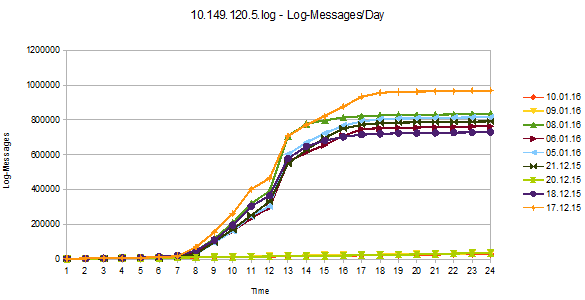
\includegraphics[scale=0.85]{img/DayAbsLogMsg.png}
\caption{Zunahme der Größe von Logdateien eines Netzwerk-Endgeräts innerhalb eines Tages}
\end{figure}
Und weiterer Inhalt...


\subsection{Kapitel 1 | Unterkapitel 2}
Bla bla...


\subsection{Kapitel 1 | Unterkapitel 3}
Noch mehr bla bla...


\section{Kapitel 2}
\subsection{Kapitel 2 | Unterkapitel 1}
''Direktes Zitat.''\cite{Zitat09}\\


\subsection{Kapitel 2 | Unterkapitel 2}
Der Begriff des 'Data Mining' wird von Jürgen Cleve und Uwe Lämmel folgendermaßen erläutert: ''Direktes Zitat 2 mit Seitenangabe.'' \cite[p. 2]{Zitat01} \\


\subsection{Kapitel 2 | Unterkapitel 3}
Der Median ist ein Lagemaß, der den mittleren Wert einer der Größe nach sortierten Messreihe angibt. Demnach ist mindestens die eine Hälfte der Messdaten kleiner gleich dem Median und mindestens die andere Hälfte größer gleich dem Median. (Vgl. \cite[p. 23]{Zitat03})\\
Das bedeutet auch, dass der Median robust gegen Ausreißern ist, da ''mindestens die Hälfte (d.h. die Mehrheit) aller Beobachtungen geändert werden müsste, um ihn beliebig zu verfälschen.''\cite[p. 27]{Zitat03}\\
Es gilt für eine geordnete Datenreihe $x_{1}$, $x_{1}$, $x_{1}$, ... , $x_{n-1}$, $x_{n}$
\\
$x_{med}$ = x[$\frac{n+1}{2}$] $\Rightarrow$ n ungerade \\
$x_{med}$ = $\frac{1}{2}$(x[$\frac{n}{2}$]+x[$\frac{n}{2+1}$]) $\Rightarrow$ n gerade. 


\bibliographystyle{amsalpha}
\bibliography{lit/lit}


\newpage
\appendix


\section{Anhang 1}


\subsection{Anhang 1 | Subanhang 1}


\subsubsection{Anhang 1 | Subanhang 1 | Subsubanhang 1} für die Tagesstunden des Montag
\begin{figure}[!htb]
	\centering
	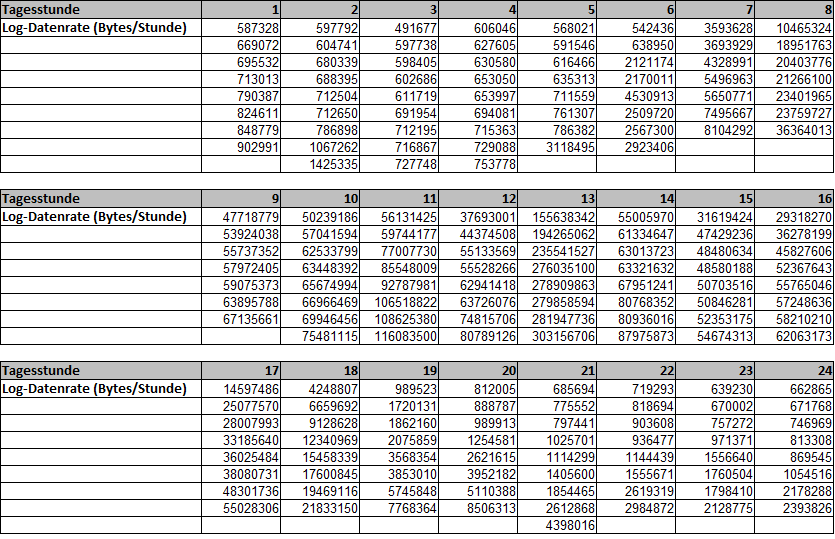
\includegraphics[scale=0.65]{img/BoxplotMessdatenPic1.png}
\end{figure}
\newpage


\subsubsection{Anhang 1 | Subanhang 1 | Subsubanhang 2} für die Tagesstunden des Montag
\begin{figure}[!htb]
	\centering
	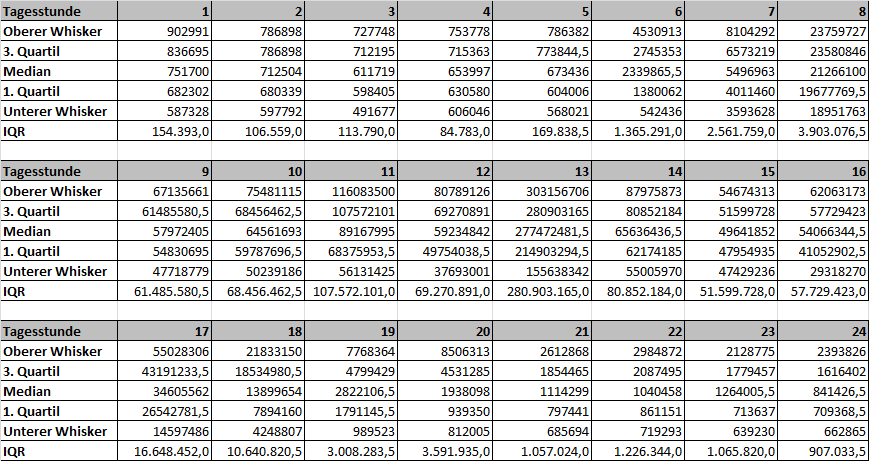
\includegraphics[scale=0.65]{img/BoxplotDatenPic1.png}
\end{figure}


\end{document}
